\section{Experiments}
\label{sec:exp}

This section presents experimental results using our approach to compute a function for the \textit{unknown component} for circuits used in cryptography.
We compare results of our implementation against the incremental SAT-based approach presented in~\cite{fujita:2015}.
The approach presented in~\cite{fujita:2015} is implemented using PICOSAT~\cite{picosat}. The experiments were performed on a 4.0GHz 
Intel(R) $\text{Core}^{\text{TM}}$ i7-6700K Quad-Core CPU with 32 GB of RAM. The data-path sizes {$k$} are selected according to cryptography standards recommended by U.S. National Institute of Standards and Technology (NIST). 
% In our experiments, the labels $NO$, $NM$, and $NI$ denote 
% % the location of unknown component within the circuit topology. Here $NI$, $NM$, and $NO$ 
% that the unknown component is near the input, middle, and near the output, respectively.
We have performed experiments for the cases when the {\it unknown component} is present near 
the input, middle, or near the output, represented using labels $NI$, $NM$, and $NO$ respectively.

\subsection{Word level specification v/s Gate level implementation}
~\autoref{masvsspec} presents the results of our approach with the {\it unknown component} 
in the Mastrovito multiplier and specification is a word level polynomial $f$. 
A Mastrovito multiplier has word level specification $Z = A\times B \pmod{ P(x)}$ 
where $P(x)$ is a given primitive polynomial for the datapath size $k$. The product $A \times B$ 
is computed using an array multiplier architecture, and then the result is reduced modulo $P(x)$. 
The circuit implementation is modeled as a set of polynomials $F=\{f_1,\dots f_i,\dots,f_s\}$. The 
approach then follows the partial reduction of specification polynomial $f$ until leading term of $f_i$ while
recording the intermediate quotients and remainders. We then represent the partial remainder as a linear combination
using the remaining gate polynomials and the quotient, to obtain the solution $P$. We 
are able to verify and compute a function for an {\it unknown component} upto 64-bits within our stipulated $TO$ (Time Out) period.

\begin{table}[H]
\centering
\caption{{Resolving Unknown Component in Mastrovito circuit against word level specification}. Time is in seconds; $k$ = Datapath Size, \#Gates = No. of gates, K = $10^3$}
\label{masvsspec}
\begin{tabular}{| c | c | c | c | c |} \hline
\multirow{2}{*}{\textbf{k}}& \#Gates & \multicolumn{3}{ c |}{Our implementation~(\autoref{sec:theory})}\\ \cline{3-5}
&&{\it NO}&{\it NM}&{\it NI}\\ \hline
9& 0.23K &00.04 & 00.04 & 00.06\\ \hline
10& 0.29K &00.09 & 00.08 & 00.08\\ \hline
11& 0.35K &00.11 & 00.10 & 00.10\\ \hline
12& 0.97K &00.47 & 00.42 & 00.43\\ \hline
13& 0.82K &00.24 & 00.23 & 00.25\\ \hline
16& 1.8K &01.08 & 01.03 & 01.07\\ \hline
32& 5.4K &150.30 & 47.28 & 42.46\\ \hline
64& 21.8K &10020.50 & 2575.71 & 2432.25\\\hline
\end{tabular}
\end{table}

Since the SAT-based approach cannot be applied against a word level specification polynomial, 
we perform experiments while using another multiplier implementation as the specification.
% The following example demonstrates the Mastrovito multiplier computation~\cite{lv:tcad2013}.
%take $\{A,B\} =
%\{a_0,a_1,\dots,a_{k-1},b_0,b_1,\dots,b_{k-1}\}$ as $k$-bit inputs and
%produce $Z = \{z_0,z_1,\dots,z_{k-1}\}$ as $k$-bit output. The multiplier
%performs $Z = A \times B \pmod{P}$, 
%The procedure 
%involves computing the product $S=A\times B$ using an array multiplier
%and then reducing it $\pmod{P}$ to obtain $Z$. We perform experiments
%on \textit{flattened} netlists of these circuits.  
% \begin{Example}
% \label{exp1}
% {\it 
% Consider the field $\mathbb{F}_{2^4}$. Let the inputs be:
% $A=a_0+a_1\cdot \alpha+a_2\cdot \alpha^2+a_3\cdot \alpha^3$ and
% $B=b_0+b_1\cdot \alpha+b_2\cdot \alpha^2+b_3\cdot \alpha^3$, and 
%  the irreducible polynomial be $P(x)=x^4+x^3+1$. 
%  % We have to perform the multiplication $Z =A\times B \pmod{ P(x) }$. 
%  The coefficients of $A = \{a_0, \dots, a_3\}, B = \{b_0, \dots, b_3\}$ are in
% $\mathbb{F}_2 = \{0, 1\}$. First, we perform the multiplication as:
% %\vspace{-0.2in}
% \vspace{0.05in}
% {\small
% {\begin{tabular}{c c c c c c c c}
% %\vspace{-0.2in}
%   &   &   & $a_3$ & $a_2$ & $a_1$ & $a_0$  \\ 
%  $\times$&   &   & $b_3$ & $b_2$ & $b_1$ & $b_0$  \\ 
%  \hline
%  &   &   & $a_3\cdot b_0$ & $a_2 \cdot b_0$ & $a_1\cdot b_0$ & $a_0\cdot b_0$ \\
%  &  & $a_3\cdot b_1$ & $a_2\cdot b_1$ & $a_1 \cdot b_1$ & $a_0\cdot b_1$ &   \\
%  & $a_3\cdot b_2$ & $a_2\cdot b_2$ & $a_1\cdot b_2$ & $a_0\cdot b_2$ &  &   \\
%  $a_3\cdot b_3$ & $a_2\cdot b_3$ & $a_1\cdot b_3$ & $a_0\cdot b_3$ &  &  &   \\
%  \hline
%  $s_6$& $s_5$  & $s_4$  & $s_3$ & $s_2$  & $s_1$   & $s_0$ 
% % \vspace{-0.2in}
% \end{tabular}}
% }
% \vspace{0.05in}
% The result $Sum = s_0+s_1\cdot \alpha + s_2\cdot \alpha^2 + s_3\cdot
% \alpha^3 + s_4\cdot \alpha^4 + s_5\cdot \alpha^5 + s_6\cdot \alpha^6$,
% where, $s_0  =  a_0\cdot b_0, ~~s_1  =  a_0\cdot b_1 + a_1\cdot b_0,
% ~~s_2 = a_0\cdot b_2 + a_1\cdot b_1 + a_2\cdot b_0$, and so on. Here
% the multiply ``$\cdot$'' and add ``$+$'' operations are performed
% modulo 2, and hence implemented in a circuit using AND and XOR
% gates. As the coefficients are always reduced modulo $p =
% 2$, there are no carry-chains
% in the design. Next, the result is reduced modulo the primitive
% polynomial $P(x) = x^4 + x^3 + 1$, as:
% % where the final output of the circuit is denoted by $G(x)  = g_3x^3
% % + g_2x^2 +g_1x + g_0$.  
% \vspace{0.05in}
% {\small
% {\begin{tabular}{|c c c c | l }
%   $s_3$   &$s_2$    &$s_1$   &$s_0$   &   \\
%  \hline
%  $s_4$    &$0$    &$0$   &$s_4$   &$s_4\cdot \alpha^4 \pmod{P(\alpha)} = s_4 \cdot (\alpha^3 + 1)$\\
%  $s_5$    &$0$    &$s_5$   &$s_5$     &$s_5\cdot \alpha^5 \pmod{P(\alpha)} = s_5\cdot (\alpha^3+ \alpha + 1)$\\
%  $s_6$    &$s_6$    &$s_6$   &$s_6$     &$s_6\cdot \alpha^6 \pmod{ P(\alpha)} = s_6\cdot( \alpha^3 + \alpha^2 + \alpha + 1)$\\
%  \hline
%  $z_3$    &$z_2$    &$z_1$   &$z_0$   &
%  \end{tabular}\par}
% }
% \vspace{0.05in}
% The final output of the circuit is: $Z = z_0 + z_1 \alpha + z_2
% \alpha^2 + z_3 \alpha^3$; where  $z_0=s_0+s_4+s_5+s_6; ~~z_1=s_1+s_5+s_6;
% ~~z_2=s_2+s_6; ~~z_3=s_3+s_4+s_5+s_6$. 
% }
% \end{Example}
\subsection{Specification and implementation as gate level circuits}

\subsubsection{Mastrovito v/s Montgomery}
\begin{figure}[H]
  \centering
  %\def\svgwidth{340pt}
  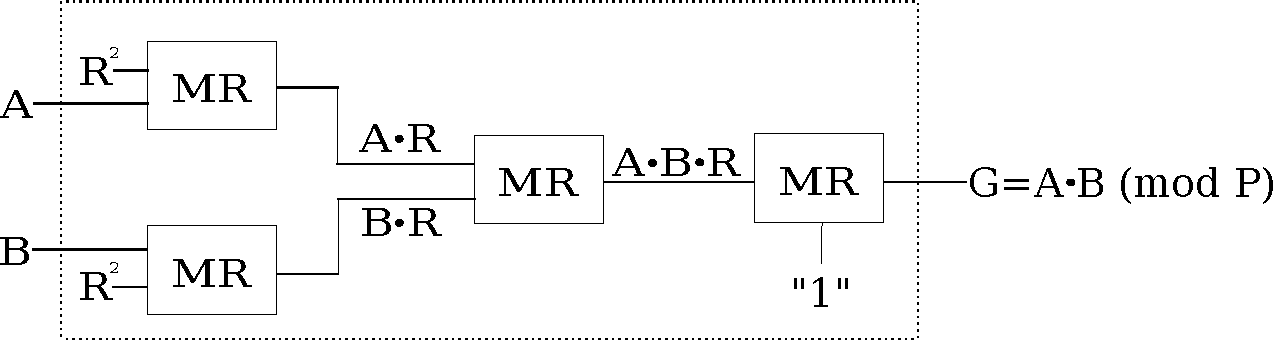
\includegraphics[scale=0.34]{new_mmcircuit-eps-converted-to}
  \caption{Montgomery multiplication.}
  \label{montfig}
  \end{figure}
Montgomery architectures~\cite{acar:1998},~\cite{wu:2002},
% \cite{Barrett:1987} 
~\cite{knezevic:2008} are considered more efficient than Mastrovito multipliers for exponentiation, 
as they do not require explicit reduction modulo $P(x)$ after each step.
~\autoref{montfig} shows the structure of a Montgomery
multiplier. Each MR block computes $A\cdot B\cdot R^{-1}$, where $R$
is selected as a power of a base ($\alpha^{k}$) and $R^{-1}$ is the multiplicative 
inverse of $R$ in $\mathbb{F}_{2^k}$. As this operation cannot compute $A\cdot B$
directly, we need to pre-compute $A\cdot R$ and $B\cdot R$ as shown in the~\autoref{montfig}. 
We denote the leftmost
two blocks as Block A (upper) and B (lower), the middle block as Block
C and the output block as Block D.
% We have presented results for GBR
%on both \textit{flattened} and \textit{hierarchical} netlists of these
% multipliers.

~\autoref{masusmontspec} presents the results of our approach with an unknown component placed in the Mastrovito multiplier with a Montgomery multiplier circuit used as the specification. While the approach~\cite{fujita:2015} finds a satisfying transformation assignment which can be mapped to a library gate, our approach computes a function which can be implemented as a single gate or sub-circuit. As shown in the table, our approach shows improvement by several orders of magnitude.

\begin{table}[H]
\centering
\caption{{Resolving Unknown Component in Mastrovito circuit with Montgomery circuit as specification}. Time is in seconds; $k$ = Datapath Size, \#Gates = No. of gates, (TO): Time-Out = 3 hrs, K = $10^3$}
\label{masusmontspec}
\begin{tabular}{| c | c |  c | c | c | c | c | c |} \hline
\multirow{3}{*}{\textbf{k}}& \#Gates & \multicolumn{3}{ c |}{Incremental SAT\textbf{~\cite{fujita:2015}}}& \multicolumn{3}{ c |}{Our Approach (\textbf{\autoref{sec:theory}})}\\ \cline{3-8}
&&{\it NO}&{\it NM}&{\it NI}&{\it NO}&{\it NM}&{\it NI} \\ \hline
9& 0.6K &33.7&36.8&34.9& 00.16 & 00.18 & 00.18\\ \hline
10& 0.7K &214.3&215&231.4& 00.28 & 00.29 & 00.40\\ \hline
11& 0.9K &1,999.5&1,927&2,090.7& 00.49 & 00.49 & 00.63\\ \hline
12& 1.6K &24,085&23,400& 8,676& 01.49 & 01.68 & 02.26\\ \hline
13& 1.7K & TO&TO&TO& 02.27 & 02.29 & 02.37\\ \hline
16& 3K &TO&TO&TO& 13.02 & 15.07 & 26.07\\ \hline
32& 9.8K &TO&TO&TO& 1204.03 & 1289.46 & 1870.42\\ \hline
\end{tabular}
\end{table}

% \subsection{Point Addition over Elliptic Curves}
% Point addition is an important operation required for the task of encryption, decryption 
% and authentication in Elliptic Curve Cryptography (ECC). 
% Modern approaches represent the points in projective
% coordinate systems, {\it e.g.}, the L$\acute{o}$pez-Dahab (LD) projective coordinate, due to which the point addition 
% operation can be implemented as polynomials in the field. 

\subsubsection{Agnew's SMPO v/s RH-SMPO}

The designs discussed so far are combinational implementations of multiplication. 
These designs use the standard basis representation $\{1,\alpha,\alpha^2, \dots,
\alpha^{k-1}\}$ to model a $k$-bit data-word $Z$ in terms of its
constituent bits as $Z = z_0 + z_1 \alpha + z_2 \alpha^2 \cdots +
z_{k-1} \alpha^{k-1}$, with $\alpha$ being the primitive element for
that field $\mathbb{F}_{2^k}$. 

\par 
%The size of the multipliers presented in the above sections
%become prohibitively large as $k$ increases.  
There exist sequential multipliers where $k$-bit inputs are loaded into $k$-bit registers,
and the $k$-bit result is available  after $k$ clock-cycle execution
of the machine. These multipliers use a {\it normal basis}
$\{\beta,\beta^{2},\beta^{4},\dots,\beta^{2^{k-1}}\}$ to  represent a
$k$-bit data-word $S$ in terms of its constituent bits as $S =
s_0\beta + s_1\beta^{2} + s_2\beta^{4} \cdots s_{k-1}\beta^{2^{k-1}}$,
with $\beta$ being the normal element and $\beta=\alpha^m$ for some $m$. 

We have performed experiments for two types of sequential multipliers namely 
Agnew's SMPO~\cite{agnew1991implementation} and RH-SMPO~\cite{RHmulti}, where the 
{\it unknown component} is in the $k$-bit unrolled Agnew's SMPO circuit, and $k$-bit 
RH-SMPO is used as the specification. The results of this experiment are 
presented in~\autoref{RHagnew}.

\begin{table}[H]
\centering
\caption{{Resolving Unknown Component in Agnew's SMPO circuit against RH-SMPO circuit implementation}. Time is in seconds; $k$ = Datapath Size, \#Gates = No. of gates, K = $10^3$}
\label{RHagnew}
\begin{tabular}{| c | c | c | c | c |} \hline
\multirow{2}{*}{\textbf{k}}& \#Gates & \multicolumn{3}{ c |}{Our implementation~(\autoref{sec:theory})}\\ \cline{3-5}
&&{\it NO}&{\it NM}&{\it NI}\\ \hline
18& 2K &01.60 & 01.63 & 01.82\\ \hline
33& 6.7K &97.14 & 100.03 & 102\\ \hline
51& 16K &1320 & 1356 & 1410\\ \hline
\end{tabular}
\end{table}

We are working on further improving the experiments by employing better data structures like
ZBDDs~(\cite{minato:zbdd}), and devising better heuristics to represent the
partial remainder as a linear combination of an ideal.